\documentclass[journal]{IEEEtran}
\usepackage{amsfonts}
\usepackage{cite,graphicx,amsmath,amsthm}
\allowdisplaybreaks[4]
\usepackage{subfigure}
\usepackage{fancyhdr}
\usepackage{dsfont}
\usepackage{array,color}
\usepackage{bm}
\usepackage{booktabs}
\usepackage{multirow}
\usepackage{algorithm}
\usepackage{algpseudocode}
\renewcommand{\qedsymbol}{\rule{0.7em}{0.7em}}
\usepackage{bbm}
\usepackage{graphicx}

\newtheorem{theorem}{Theorem}
\newenvironment{theorembox} {\begin{theorem}}{\hfill \interlinepenalty200 $\Box$\end{theorem}}
\newtheorem{lemma}{Lemma}
\newenvironment{lemmabox} {\begin{lemma}}{\hfill \interlinepenalty500 $\Box$\end{lemma}}
\newtheorem{proposition}{Proposition}
\newenvironment{propositionbox} {\begin{proposition}}{\hfill \interlinepenalty500 $\Box$\end{proposition}}
\newtheorem{corollary}{Corollary}
\newenvironment{corollarybox} {\begin{corollary}}{\hfill \interlinepenalty500 $\Box$\end{corollary}}
\newtheorem{property}{Property}
\newenvironment{propertybox} {\begin{property}}{\hfill \interlinepenalty500 $\Box$\end{property}}
\newtheorem{remark}{Remark}
\newenvironment{remarkbox} {\begin{remark}}{\hfill \interlinepenalty500 $\Box$\end{remark}}
\newtheorem{claim}{Claim}
\newenvironment{claimbox} {\begin{claim}}{\hfill \interlinepenalty500 $\Box$\end{claim}}


\begin{document}
\title{{\huge An algorithm of adaptive Matrix Multiplication based on Strassen's method}}
\author{Pengzhan Jiang$^{*\diamond}$, Yiyang Zhang$^{*\diamond}$, Buyi Li$^{*\diamond}$, Jinyu Wu$^{*\diamond}$,\\
        $^{*}$Department of Electrical and Electronic Engineering, \\$^{*\diamond}$Southern University of Science and Technology, Shenzhen 518055, China\\
E-mail: \{11811003, 11811523, 11810709, 11810838\}@mail.sustech.edu.cn
}


\maketitle
\begin{abstract}
 Strassen’s matrix multiplication (MM) has benefits with respect to any (highly tuned) implementations of MM because Strassen’s reduces the total number of operations.
 Strassen used matrix addition (MAs) instead of MMs to reduce the amount of computation.
 But the traditional Strassen's method is a divide and conquer method.
 It divides an $\mathrm{N} \times \mathrm{N}$ matrix into four $\mathrm{N}/2 \times \mathrm{N}/2$ parts and recurses.
 Therefore, when the matrix order is not a power of 2, recursion will report an error.


 In this paper, we will implement and analyze, empirically and theoretically, a method for multiplying square matrices.
 We will first write pseudocode for Strassen’s algorithm and the standard square matrix multiply algorithm that runs in $\theta(n^3)$.
 Then extend the pseudocode of Strassen’s algorithm so that it will work with any value of n (not just n that is a power of 2) and give a complete a proof of the Asymptotic bounds for the runtime of Strassen’s algorithm and square matrix multiply.
 Finally, we will implement the standard Square Matrix Multiply, $\theta(n^3)$, algorithm for matrix multiplication and Strassen’s matrix multiplication algorithm.
\end{abstract}


\begin{IEEEkeywords}
Strassen's method, matrix multiplication, adaptive method.
\end{IEEEkeywords}



\section{Introduction}
Matrix multiplication is one of the most basic operations in linear algebra and scientific computing, which is widely used but extremely time-consuming.
Improving the computing speed of matrix is conducive to reducing the time consumption of many computational problems in scientific and engineering fields.
A lot of matrix multiplication is often involved in the calculation of various scientific research and engineering problems.
Therefore, improving the computational efficiency of matrix multiplication is the key to many computational problems and also an important field of algorithm design and research.
Many computer scientists have done a lot of work in this area.


In this paper, Strassen algorithm is used to implement and improve, and its time complexity is analyzed and discussed, and the applicable scope of this algorithm is summarized.
Strassen algorithm for matrix multiplication is modified first.
It can also be used for matrices that do not have to be powers of 2.
Also, give a complete a proof of the Asymptotic bounds for the runtime of Strassen’s algorithm and square matrix multiply.
Moreover, the Strassen algorithm is improved to set a limit.
Because Strassen algorithm is used in this paper for recursive operation, a large number of dynamic two-dimensional arrays need to be created, in which allocating heap memory space will occupy a large amount of computing time, thus masking the advantages of Strassen algorithm.
When n$<$bounds, the matrix is computed using the common law instead of continuing divide-and-conquer recursion.
Different environments (hardware configuration) have different boundaries.
Generally speaking, matrix multiplication is processed faster by naive method.
Strassen algorithm is considered only when the matrix becomes denser and the order of the matrix is large.


In this paper, the conventional method of matrix multiplication and Strassen algorithm were successfully implemented, and the defects of Strassen algorithm when using dynamic memory allocation were found and improved.
It is also found that Strassen algorithm consumes a lot of memory and has to make a proper trade-off when using space for time.
\section{background}
1969, Volker Strassen prove $\Theta(N^3)$ is not the solution to the optimal algorithm of matrix multiplication.
He did eventually put forward a series of work for the first time complexity is lower than $\Theta(N^3)$ matrix multiplication algorithm.
The algorithm complexity is $\Theta(n^{\mathrm{log}_27})=\Theta(n^{2.807})$.


In 2004 a theoretical computer scientist and a mathematician came up with a promising new approach to group theory for fast matrix multiplication, as demonstrated by two researchers, Chris Umans of the California Institute of Technology (CIT) and Henry Cohn of Microsoft Research.
If there are groups that satisfy both conditions, the group theory method produces a nontrivial ($<3$) upper bound on the matrix multiplication index.
In 2006, Mr Cohn and Mr Umans, together with Robert Kleinberg at the University of California, Berkeley, and Balazs Szegedy at the Princeton Institute for Advanced Study, found groups that met both conditions.
In a recent paper, four collaborators describe a series of new algorithms for matrix multiplication, the most efficient of which can match the running time of the fastest known algorithm, and propose two hypotheses.
Each guess affirmation answer contains the index of matrix multiplication is 2.
As soon as Mr. Kleinberg said, “our approach makes the connection between the fast matrix multiplication and group theory obviously, this could give us more research tools.”


Strassen's algorithm recalls a shortcut to complex multiplication that Gauss first observed.
Although the product $(a+ bi)(c+di) =ac-bd+(bc+ad)i$ which seems to require four multiplications, Gauss observed that this can actually be done with three multiplications, namely $ac$, $bd$ and $(a+b)(c+d)$, because $bc+ad=(a+b)(c+d)-ac-bd$.
Similarly, Strassen's algorithm reduces the number of multiplications required to compute the product of two $2\times2$ matrices A and B from eight to seven by expressing the elements of AB as linear combinations of the products of linear combinations of elements of A and B.


This-after applying the technique to the 4 blocks of the $2N\times2N$ matrix, reduces the problem to multiplication of seven $2^{n-1}\times 2^{n-1}$ matrices.
Recursively using this method, the algorithm for running time $\Theta(n^{\mathrm{log}_27})=\Theta(n^{2.807})$ is given.
Strassen application partition method, by putting the problem is decomposed into smaller subproblems, the smaller the subproblem then built, will have solve the problem of child merger, finally it is concluded that the parent solution of the problem.
This idea can greatly reduce the algorithm complexity, because the complexity of matrix multiplication is mainly reflected in multiplication, and one or two more additions will not increase the complexity too much.

\section{theoretical analysis}
From the previous theory, we deduced that the time complexity of Strassen's method algorithm is $\Theta(n\mathrm{log}_27)$, which is obviously less than the complexity of the direct algorithm $\Theta(N^3)$.
However, through many experiments, it can be observed that when n is less than a certain value, the direct algorithm is faster than Strassen's method in calculation.
By comparing the algorithm steps, we can sum up the following reasons.


1) Strassen method uses a high constant, which has a better effect on typical application of naive method.


2) For sparse matrices, there are better methods specially designed for them.
The submatrices in the recursion take up extra space.


3) The error accumulation of Strassen algorithm is larger than that of the naive method due to the limited computing accuracy of non-integral values.
Here we assume the reason is not about the error.

\begin{align}
  T(\mathrm{n})=
  \begin{cases}
    O(1)& \text{n=2}\\
    7T(n/2)+O(n^2)& \text{n\textgreater 2}
    \end{cases}
\end{align}


Here we need to go back to the original analysis and we identify size of a matrix $\mathcal{A}\in :\mathcal{M}^{m\times n}$ as

\begin{align}
  \sigma(\mathrm{A})= m* n \\
  C=A*B
\end{align}

For naive method
\begin{align}
  C_0 = A_0B_0 + A_1B_2,\\
  C_1 = A_0B_1 + A_1B_3,\\
  C_2 =A_2B_0 + A_3B_2,\\
  C_3 = A_2B_1 + A_3B_3.
\end{align} 
Thus, for every matrix element $C_i(0\leq i\leq 3)$, the classical approach computes two products, for a total of 8 Matrix Multiplications and 4 Matrix Additions.


As for Strassen’s method,

\begin{align}
  C_0=M_1+M_4-M_5+M_7,\\
  C_1=M_2+M_4,\\
  C_2=M_3+M_5,\\
  C_3=M_1+M_3-M_2+M_6,\\
  M_1=T_0T_1,\\ 
  T_0=A_0+A_3,\\
  T_1=B_0+B_3,\\
  \sigma(T_0) = \sigma(T_1) = \sigma(M_1) = [n] \times [n],\\ 
  M_2 = T_2B_0,\\
  T_2 = A_2 + A_3,\\ 
  \sigma(T_2) = \sigma(M_2) = [n] \times [n] 
  M_3 = A_0T_3,\\
  T_3 = B_1 + B_3,\\ 
  \sigma(T_3) = \sigma(M_3) = [n] \times [n],\\ 
  M_4 = A_3T_4,\\
  T_4 = B_2-B_0,\\
  \sigma(T_4) = \sigma(M_4) = [n] \times [n],\\
  M_5 = T_5B_3,\\
  T_5 = A_0 + A_1,\\
  \sigma(T_5) = \sigma(M_5) = [n] \times [n],\\
  M_6 = T_6T_7,\\
  T_6 = A_2 - A_0,\\
  T_7 = B_0 + B_1,\\
  \sigma(T_6) = \sigma(M_6) = [n] \times [n],\\
  M_7 = T_8T_9,\\
  T_8 = A_1 - A_3,\\
  T_9 = B_2 + B_3,\\
  \sigma(T_8) = [n] \times [n],\\
  \sigma(T_9) = [n] \times [n],\\ 
  \sigma(M_7) = [n] \times [n]
\end{align}


From equation (8) to equation (36), we can know that our implementation requires 22 matrix updates (4 copies and 18 additions) and 7 recursive calls.
Thus, a tentative cross-over size is the size for which the work of the 22 Matrix Additions is equal to the one (avoided) of a single MM:$2(m/2)^3=22(m/2)^2$,
that is $m = 22$.
This cross-estimation is based on the bottom-up approach and is not really accurate.


In other words, $l$ is the number of times we execute it.
The decomposition of the problem, or the expansion of the function, in which case the difference between the cost of preserving multiplication and the cost of adding is greatest.
In practice, a more precise analysis would suggest stopping recursion at level $l\geq 1$ so that
\begin{align}
  \max _{\ell>0}\sum_{k=0}^{\ell-1}\left(\frac{7}{4}\right)^{k}\left[\frac{n}{2^{k+1}} \pi_{\frac{n}{2^{k+1}}} - \alpha_{\frac{n}{2^k}}\right]
\end{align}

Assume $\alpha n$ is for Matrix Addition(Matrix copy has the same coefficient) for matrices of size $n \times n$ and $\pi n$ is the efficiency coefficient for Matrix Multiplication.
Thus, for problems of size smaller than $n_1$, Strassen’s algorithm should be avoided;
for problems of size $(l)n_1 \leq n < (l+ 1)n_1$, we may apply Strassen’s ` times.
for the naive method needs $n^3$, Assume $\alpha$ and $\pi$ are constant, the cross over point can be calculate by

\begin{align}
  n>11\frac{\alpha}{\pi} 2^l
\end{align}
Of course, the ratio $\pi/\alpha$ is machine and problem size dependent.
 The following chart is the experimental value of several systems.\cite{pro1}
 If we assume a ratio $\alpha/\pi = 50$ (i.e. common for the systems adopted in this work when the matrices lie in memory only), we find that the cross-over size is $n_1 > 1100$.
 Thus, for problems of size smaller than $n_1$, Strassen’s algorithm should be avoided we need to use naive method.

 \begin{figure}[h]
	\centering
	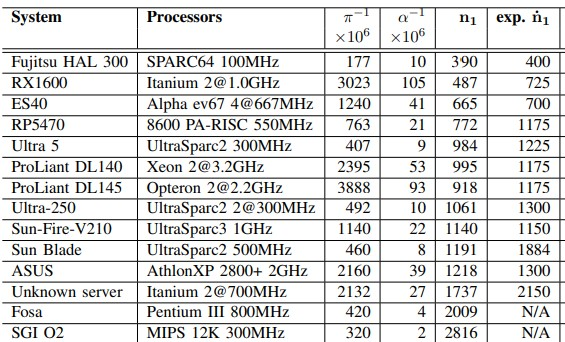
\includegraphics[width=70mm]{./img/Fig2.jpg}
	\caption{Systems and performance:$\frac{1}{\pi}10^6$ is the performance of cblas dgemm or DGEMM (GotoBLAS) in MFLOPS for $n=1000$;$\frac{1}{\alpha}10^6$is the performance of MA in MFLOPS for $n=1000$;$n_1$ is the theoretical recursion point as estimated in $22\frac{\alpha}{\pi}$;instead,$n_1$ is the measured recursion point.}
	\label{fig_sim}
\end{figure}

\section{methodology}

\setcounter{secnumdepth}{4}
\subsection{Strassen algorithm and its extension}
Let's consider a matrix $C=AB$, where $A$ and $B$ are $\mathrm{n}\times\mathrm{n}$ matrices.
According to the definition of matrix multiplication, each element in $C$ needs to be calculated as follows
\begin{align}
&c_{ij}=\sum_{k=1}^{n}a_{ik}b_{kj},\label{cij}
\end{align}
This equation contains N times for loop, so the time complexity of calculating $c_{ij}$ is $\Theta(n)$.
Matrix $C$ has $n^2$ elements, so the total time complexity is $\Theta(n^3)$. 
When $n$ is large, even the computer can not afford such a computing time.
However, with the wisdom of scientists, people gradually found that there are some matrix multiplication algorithms lower than $\Theta(n^3)$.
Strassen is a pioneer in this field.
He took the lead in reducing the time complexity of matrix multiplication to $\Theta(n^{\mathrm{lg}7})\approx \Theta(n^{2.81})$.
Don't underestimate this subtle improvement, when n is very large, the algorithm will save a lot of time than ordinary algorithm.


Strassen's algorithm and its variants are called the most efficient matrix multiplication methods.
It reduces the number of scalar multiplications involved in the computation of a matrix multiplication. 
This is achieved by replacing a large matrix multiplication with a combination of smaller matrix multiplications and matrix additions.
These smaller multiplications can also be subdivided using the algorithm recursively.


Strassen divides each $\mathrm{n}\times\mathrm{n}$ matrix into four $\mathrm{n}/2 \times \mathrm{n}/2$ matrices.
We rewrite the matrices $A$, $B$ and $C$ as follows.
\begin{align}
A={
  \left[ \begin{array}{ccc}
    A_{11} & A_{12} \\
    A_{21} & A_{22}  
    \end{array} 
    \right ]
},B={
  \left[ \begin{array}{ccc}
    B_{11} & B_{12} \\
    B_{21} & B_{22}  
    \end{array} 
    \right ]
},C={
  \left[ \begin{array}{ccc}
    C_{11} & C_{12} \\
    C_{21} & C_{22}  
    \end{array} 
    \right ]
}\label{A}
\end{align}
So $C=AB$ can be rewritten as 
\begin{align}
  &C={
  \left[ \begin{array}{ccc}
    C_{11} & C_{12} \\
    C_{21} & C_{22}  
    \end{array} 
    \right ]
}={
  \left[ \begin{array}{ccc}
    A_{11} & A_{12} \\
    A_{21} & A_{22}  
    \end{array} 
    \right ]
}{
  \left[ \begin{array}{ccc}
    B_{11} & B_{12} \\
    B_{21} & B_{22}  
    \end{array} 
    \right ]
}
\end{align} 


Then create the following 10 intermediate matrices.
\begin{align}
&S_1=B_{12}-B_{22},
&S_2=A_{11}+A_{12},\notag
& \ \ \ S_3=A_{21}+A_{22},\\ \notag
&S_4=B_{21}-B_{11},
&S_5=A_{11}+A_{22},
& \ \ \ S_6=B_{11}+B_{22},\\ \notag
&S_7=A_{12}-A_{22},
&S_8=B_{21}+B_{22},
& \ \ \ S_9=A_{11}-A_{21},\\ \notag
&S_{10}=B_{11}+B_{12}. 
\end{align} 
Calculate 7 times matrix multiplication.
\begin{align}
 &P_1=A_{11}S_1,
 &P_2=S_2B_{22},\notag
 &\ \ \ P_3=S_3B_{11}, \\\notag
 &P_4=A_{22}S_4,
 &P_5=S_5S_6,
 &\ \ \ P_6=S_7S_8,\\ \notag
 &P_7=S_9S_{10},
\end{align}
According to these seven results, we can calculate matrix $C$.
\begin{align}
  \notag
&C_{11}=P_5+P_4-P_2+P_6,\\ \notag
&C_{12}=P_1+P_2,\\ \notag
&C_{21}=P_3+P_4,\\ \notag
&C_{22}=P_5+P_1-P_3-P_7 \notag
\end{align}



So we can easily get to know the pseudocode of Strassen algorithm.
\begin{algorithm}[htb]  
  \caption{STRASSEN-MATRIX-MULTIPLY}  
   
  \begin{algorithmic}  
    \Require  
    square matrix A and B 
    \State n=A.rows
    \If{n==1}
    \State  $c_{11}=c_{11}+a_{11}*b_{11}$
    \Else
    \State divide $A_{n\times n}$, $B_{n\times n}$ and  $C_{n\times n}$  into four sub-matrices.
    \State $S_1=B_{12}-B_{22}$
    \State $S_2=A_{11}+A_{12}$
    \State$S_3=A_{21}+A_{22}$
    \State$S_4=B_{21}-B_{11}$
    \State$S_5=A_{11}+A_{22}$
    \State$S_6=B_{11}+B_{22}$
    \State$S_7=A_{12}-A_{22}$
    \State$S_8=B_{21}+B_{22}$
    \State$S_9=A_{11}-A_{21}$
    \State$S_{10}=B_{11}+B_{12}$
    \State $P_1$ = STRASSEN-MATRIX-MULTIPLY(A11,$S_1$)
    \State $P_2$ = STRASSEN-MATRIX-MULTIPLY($S_2$,B22)
    \State $P_3$ = STRASSEN-MATRIX-MULTIPLY($S_3$,B11)
    \State $P_4$ = STRASSEN-MATRIX-MULTIPLY(A22, $S_4$)
    \State $P_5$ = STRASSEN-MATRIX-MULTIPLY($S_5$ ,$S_6$)
    \State $P_6$ = STRASSEN-MATRIX-MULTIPLY($S_7$,$S_8$)
    \State $P_7$ = STRASSEN-MATRIX-MULTIPLY($S_9$,$S_{10}$)
    \State C$_{11}$=$P_5+P_4-P_2+P_6$
    \State C$_{12}$=$P_1+P_2$
    \State C$_{21}$=$P_3+P_4$
    \State C$_{22}$=$P_5+P_1-P_3-P_7$
    \State return C
    \EndIf

  \end{algorithmic}  
\end{algorithm}




Similarly, we can write the recurrence formula of Strassen algorithm.
\begin{align}
  T(\mathrm{n})=
  \begin{cases}
    O(1)& \text{n=2}\\
    7T(n/2)+O(n^2)& \text{n\textgreater 2}
    \end{cases}
\end{align}

\begin{align}
  \notag
  T(n) &=7 T\left(\frac{n}{2}\right)+O\left(n^{2}\right) \\\notag
&=7\left[7 T\left(\frac{n}{2^{2}}\right)+O\left(\left(\frac{n}{2}\right)^{2}\right)\right]+O\left(n^{2}\right) \\\notag
&=7^{2} T\left(\frac{n}{2^{2}}\right)+7 O\left(\frac{n^{2}}{4}\right)+O\left(n^{2}\right) \\\notag
&=7^{2}\left[7 T\left(\frac{n}{2^{3}}\right)+O\left(\left(\frac{n}{2^{2}}\right)^{2}\right)\right]+7 O\left(\frac{n^{2}}{4}\right)+O\left(n^{2}\right) \\\notag
&=7^{3} T\left(\frac{n}{2^{3}}\right)+7^{2} O\left(\frac{n^{2}}{4^{2}}\right)+7 O\left(\frac{n^{2}}{4}\right)+O\left(n^{2}\right) \\\notag
&=7^{3} T\left(\frac{n}{2^{3}}\right)+7^{2} O\left(\frac{n^{2}}{4^{2}}\right)+7 O\left(\frac{n^{2}}{4^{1}}\right)+7^{0} O\left(\frac{n^{2}}{4^{0}}\right) \\\notag
&=\ldots \ldots \\\notag
&=7^{k} T\left(\frac{n}{2^{k}}\right)+7^{k-1} O\left(\frac{n}{4^{k-1}}\right)+7^{k-2} O\left(\frac{n}{4^{k-2}}\right)+\ldots \\ \notag
&\ldots +7^{2} O\left(\frac{n^{2}}{4^{2}}\right)+7^{1} O\left(\frac{n^{2}}{4^{1}}\right)+7^{0} O\left(\frac{n^{2}}{4^{0}}\right) \notag
\end{align}


When $T\left(\frac{n}{2^{k}}\right)=T(2)=O(1)$ , $k=\log _{2} n-1=\log _{2}\left(\frac{n}{2}\right)$.


Also, $T(n)=O(n) \Leftrightarrow T(n) \leq c n$

\begin{align}
  \notag
  T(n) & \leq 7^{k} O(1)+c \cdot n^{2} \cdot\left(\frac{7}{4}\right)^{k-1}+c \cdot n^{2} \cdot\left(\frac{7}{4}\right)^{k-2}+\ldots\\ \notag
   &\ldots+c \cdot n^{2} \cdot\left(\frac{7}{4}\right)^{2}+c \cdot n^{2} \cdot\left(\frac{7}{4}\right)^{1}+c \cdot n^{2}\left(\frac{7}{4}\right)^{0} \\ \notag
& \leq 7^{k} \cdot c+c \cdot n^{2} \cdot\left[\left(\frac{7}{4}\right)^{k-1}+\left(\frac{7}{4}\right)^{k-2}+\ldots +\left(\frac{7}{4}\right)^{0}\right]\\ \notag
&\leq c \cdot 7^{\log _{2}\left(\frac{n}{2}\right)}+c \cdot n^{2} \cdot\left[\frac{1 \cdot\left(1-\left(\left(\frac{7}{4}\right)^{k}\right)\right)}{1-\frac{7}{4}}\right] \\ \notag
&\leq c \cdot 7^{\log _{2}\left(\frac{n}{2}\right)}+c \cdot n^{2} \cdot\left[\frac{4}{3}\left(\left(\frac{7}{4}\right)^{k}-1\right)\right] \\ \notag
&\leq c \cdot 7^{\log _{2}\left(\frac{n}{2}\right)}+c \cdot n^{2} \cdot\left[\frac{4}{3}\left(\left(\frac{7}{4}\right)^{\log _{2}\left(\frac{n}{2}\right)}-1\right)\right] \\ \notag
&\leq \frac{c}{7} \cdot 7^{\log _{2}(n)}+c \cdot n^{2} \cdot\left[\frac{4}{3}\left(\frac{4}{7}\left(\frac{7}{4}\right)^{\log _{2}(n)}-1\right)\right] \\ \notag
&\leq \frac{c}{7} \cdot 7^{\log _{2}(n)}+c \cdot n^{2} \cdot\left[\frac{16}{21}\left(\frac{7}{4}\right)^{\log _{2}(n)}-1\right]
\end{align}


Follow we proof $7^{\log _{2}(n)}=n^{\log _{2}(7)}:$
\begin{align}
  \notag
 &7^{\log _{2}(n)}=?,\\\notag
 &\log _{7}(?)=\log _{2}(n) \\\notag
&\frac{\log _{2}(?)}{\log _{2}(7)}=\log _{2}(n) \\\notag
&\log _{2}(?)=\log _{2}(n) \cdot \log _{2}(7) \\\notag
&2^{\log _{2}(?)}=2^{\log _{2}(n) \cdot \log _{2}(7)} \\\notag
&?=n^{\log _{2}(7)}
\end{align}
\begin{align}
  \notag
  T(n) & \leq \frac{c}{7} \cdot 7^{\log _{2}(n)}+c \cdot n^{2} \cdot\left[\frac{16}{21}\left(\frac{7}{4}\right)^{\log _{2}(n)}-1\right] \\\notag
& \leq \frac{c}{7} \cdot n^{\log _{2}(7)}+c \cdot n^{2} \cdot\left[\frac{16}{21}(n)^{\log _{2}\left(\frac{7}{4}\right)}-1\right] \\\notag
& \leq C \cdot n^{\log _{2}(7)}-C \cdot n^{2}
\end{align}
Finally, we get $T(n)=\Theta(n^{\mathrm{log}_27})\approx \Theta(n^{2.81})$


The previous pseudocode may have some problems when the matrix order n is not a power of 2.
So we extend the pseudocode of Strassen’s algorithm so that it will work with any value of n.
Here is the pseudocode of the adaption function
\begin{algorithm}[htb]  
  \caption{ADAPTION FUNCTION}  
   
  \begin{algorithmic}  
    \Require  
    input N(The size of the matrix)
    \If{inputN$\neq$POWER OF TWO}
    \State output N=1
    \While{ input N$>$output N}
    \State output N=output$\times$2 
    \EndWhile
    \Else 
    \State output N=input N
    \EndIf
  \end{algorithmic}  
\end{algorithm}



\subsection{standard matrix multiplication}


Suppose A is a matrix of m$\times$p and B is a matrix of p$\times$n, then the matrix C of m$\times$p is called the product of matrix A and B.
C=AB is called the matrix product.
The elements in row $i$ and column $j$ in matrix C can be expressed as follows:
\begin{align}
  (\mathrm{AB}_{ij})=\sum_{k=1}^{p}a_{jk}b_{kj}=a_{i1}b_{1j}+\cdots+a_{ip}b_{pj}
\end{align}

\begin{figure}[h]
	\centering
	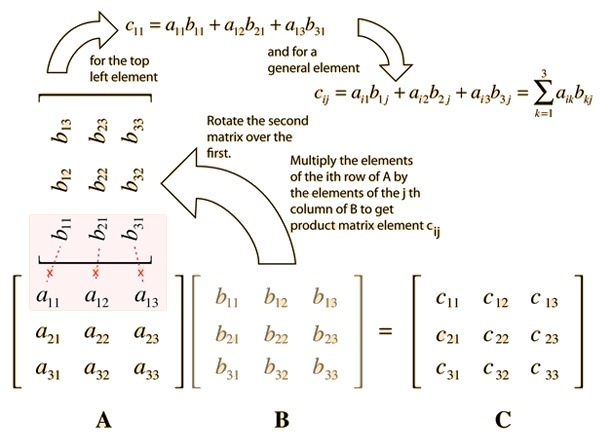
\includegraphics[width=70mm]{./img/Fig1.jpg}
	\caption{matrix multiplication}
	\label{fig_sim}
\end{figure}


If in matrix A and matrix B, $m=p=n=N$, then the number of multiplications required to complete C = AB is:
For each row vector r, there are n rows in total.
For each column vector C, there are n columns in total.
To calculate their inner product, there are $N$ multiplications in total.
It can be seen from the synthesis that the algorithm complexity of matrix multiplication is:$\Theta(n^3)$
We can also get the complexity from the pseudocode which is below.


\begin{algorithm}[htb]  
  \caption{NAIVE-MATRIX-MULTIPLY}  
   
  \begin{algorithmic}  
    \Require  
    square matrix A and B 
    \State m =A.rows 
    \State p=A.columns
    \State n = B.columns
    \State create a new $m\times n$ matrix C
    \For {i=1 to m}  
      \For{j=1 to n}
      \State $C_{ij}=0$
      \For{k=1 to p}
      \State $c_{ij}=c_{ij}+a_{ik}*b_{kj}$
      \EndFor  
      \EndFor
    \EndFor
  \end{algorithmic}  
\end{algorithm}


\subsection{run time analysis}
Before run time analysis, we should first explain that our strassen algorithm is not $n\neq 2^n$, that is, it can not be divided into two parts, we adopt the following algorithm:
For a square matrix (square matrix), find the smallest $l$ such that $l=2^k$, $k$ is an integer and $l>m$.
The rest of the blank points are filled with 0, and the square matrix with $l$ side length is adopted Strassen algorithm, and then 0 is removed.
After checking, we found that $0 \times 0$ also takes up the operation time of a multiplication, so the operation time of $2^n + 1$ to $2^{n+1}$ is the same, so we only consider $n=2^k$.


From part A, we can know that in theory, Strassen needs 18 addition and 7 multiplication.
Since the operation time of $1 \times 1$ multiplication is much longer than that of $1 \times 1$ addition, we assume that a one-time addition and subtraction $(n\pm n)$ operation is the same as multiplication $(1 \times 1)$ operation, which is counted as one operation.
Therefore, the number of operations required for the addition and subtraction of $n\times n$ matrix is $n^2$.
According to the naive method, the multiplication of $n times n$ matrix requires $n^3$ operations.
At the same time, the time of matrix splitting is not considered.
We can get the theoretical time when $n = 2^k$.


Strassen algorithm : $T_{k+1} = 18 +8T_k$, where $T_0=1$.


Naive algorithm : $n^3=2^{3k}$


Strassen algorithm is running faster after $n=1335$.

\section{experiment design}
In this experiment, we divided the whole project into 5 sub-tasks.


1. Theoretical analysis and pseudocode writing of Strassen algorithm (including its adaptive form).


2. Run time calculation of special cases based on pseudo code.


3. Java implementation of algorithm design.


4. Testing, plotting and fitting of algorithm running time.


5. Analysis of relevant conclusions.


In the process of carrying out the related experiments and completing the related experiments, we found that the experimental tasks were increased and two sub-tasks were added.


6. The running time test and analysis of the two algorithms after blocking.


7. Optimization related conclusions.


In the formal experiment process, we first complete the pseudocode, and then write the actual code according to the pseudocode.
Through the coding process of the two algorithms, we have a deeper understanding of the deep logic of the algorithm.
Especially for the writing process of Strassen algorithm, we have a deep understanding of the original theoretical Strassen algorithm running process.
For the two algorithms, we have trained the ability to write code and consolidated the theoretical knowledge.
We always think that this process helps us to improve our learning ability.


After the completion of the code, we found that Strassen algorithm is always longer than the traditional algorithm. 
In order to solve this problem, we analyze the program in blocks.
We finally found that Strassen algorithm itself can shorten the calculation time, but because of the replication of matrix and other operations in our code, the running time is prolonged.

\section{empirical analysis}
We find that the running time of Strassen algorithm is still longer than the theoretical results when $n = 1335$.
Then use JAVA program to test the run time.
\begin{figure}[h]
	\centering
	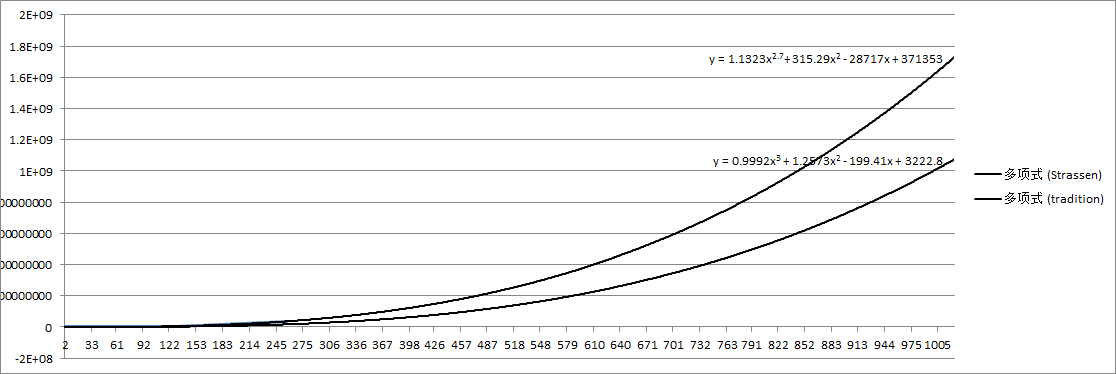
\includegraphics[width=70mm]{./img/1.png}
	\caption{Actual fitting results}
	\label{fig_sim}
\end{figure}
Then the actual measurement result $n=11324$.
There is a big gap with the theoretical value $n=1335$.
After discussion and demonstration, we decided to adopt the method of splitting, that is, to separate all parts of the algorithm.
The time spent in each part is explored by block velocity measurement.


In fact, we only need to measure the matrix operation, block, copy and other operations to get the results, but in order to better measure the actual running time of the algorithm, we measure the addition and multiplication parts of the matrix to help us further explore.


The results are as follows:


1. The addition operation is really fast. The addition speed of $8\times 8$ matrix is much faster than that of $4 \times 4$ matrix.


2. The process of matrix replication is very slow, and the time of one copy is about half of that of a multiplication operation.
Therefore, in our experiments, Strassen algorithm always takes longer than the naive algorithm, which should be caused by matrix duplication.


3. During the test, we found that the speed of addition, subtraction and multiplication increased significantly after the program was started for a period of time, but the copy speed was basically unchanged.
We analyze this problem and think that there may be two reasons.
First, when our program runs for a period of time, the CPU may allocate more space to the program.
The performance previously allocated to other programs will be more focused on this program.
This also explains why other computer programs slow down after a while.
The other is that some operation data stored in memory can be reused by the program.
But we quickly overturned this idea after demonstration.
This is because our calculation process is based on the operation of random numbers, and the matrix applied to multiplication is generated randomly.
We find that the results of the algorithm are completely correct by sampling the results of the algorithm.
Therefore, the program does not use the data stored in memory.
Therefore, we think that it is because of the CPU allocation that the program runs faster.
Therefore, in the subsequent data processing process, we adopt the scheme of ignoring the maximum 5\% and the minimum 5\% of the repeated test data to calculate the average value.
Based on the above conclusion, we find that the time required for matrix replication is about $\Theta(n^2)$.
On this basis, we have carried out 1000 experiments by changing the size of $n$. Finally, for an $n \times n$ matrix, the copy time is $(3n/4)^2$.
Then we rewrite the formula:


Strassen : $ T_{k+1}=12\times((3\times 2^k)/4)^2+7T_k + 18$, where $T_0 = 1$.


Naive : $n^3=2^{3k}$

After changing the recursive formula, we calculate the time needed for the algorithm again. 
We calculated that after $n=12411$, strassen algorithm runs faster.

\section{contributions}
This article is written in LaTeX and there may be some small mistakes.
In this project, Pengzhan Jiang is responsible for the writing of the project report and the theoretical analysis of the asymptotic bound of Strassen algorithm and naive algorithm.
Yiyang Zhang is responsible for data collection, project background analysis and pre-experiment design.
Buyi Li is responsible for the implementation and extension of Strassen algorithm on Java IDEA.
Jinyu Wu is responsible for runtime analysis and the choice of Strassen algorithm and naive algorithm.

\section{Conclusions}


This paper has studied the Strassen algorithm and its adaption.
Through this experiment, we found that the Strassen algorithm can significantly reduce the time required for matrix operation, so as to achieve the effect of optimizing the matrix operation process.
In the previous part, we show the time spent by Strassen algorithm and traditional matrix operation method in the form of chart.
The conclusion obtained from the experiment is basically consistent with our theoretical analysis, so this experiment was successfully completed.
In the experiment, we divided the program separately and studied the specific running time of each part.
Through this process, we find that the operation time of Strassen algorithm is shorter than that of traditional algorithm.
In the first half of the experiment, Strassen algorithm takes a long time because our program adds extra cost to the algorithm.


\section{what we have learnt}
This is the end of the experiment.
We have gained a lot in the experiment.
After discussion, we have found three points.


First, through experiments, we really realized the process of turning the algorithm learned in a book into a program.
The programs we wrote in the previous study are relatively elementary, and they are not as complicated as Strassen algorithm.
The process of programming is a good exercise of our ability to write programs, exercise our logic.
At the same time, for Strassen algorithm to complete the programming process also let us further understand the underlying logic of the algorithm.


Secondly, in this experiment, we also designed the pre-experiment part.
We study the convenience of matrix multiplication through the pre-experiment. Although the pre-experiment is not directly related to our Strassen algorithm, the pre-experiment further helps us understand the advantages of the matrix operation process than the linear algorithm.
Through the pre-experiment, we have a good grasp of the underlying architecture of matrix operation, and have a deeper understanding of the application of matrix operation in Strassen algorithm.
The design of the pre-experiment itself has brought us great harvest.
In the previous experiment process, we are based on the experimental requirements of the part to complete the experiment.
This kind of experiment is safe and will not make mistakes.
But through the experiment can bring the harvest is very limited.
In the pre-experiment part of this experiment, we have greatly developed our learning initiative through active design.
In the process of pre experiment, we encountered many difficulties and explored in the process of continuous failure, but we did not give up the part of pre experiment, and finally completed the experiment successfully.


Finally, we get the conclusion of the experiment through the partition procedure.
After we have completed the code programming of Strassen algorithm, the experimental results are not consistent with the theoretical analysis.
We studied it for a long time without finding the cause.
In the end, we propose a scheme to separate the program. By dividing the program into a sub part, we can study it separately.
We measure the running time of the two algorithms separately through the process of splitting, and the final results are consistent with the theoretical analysis.
This proves that our program is completely correct.
It is a good idea for this experiment to measure the time by splitting the program.
We think this is the biggest gain we obtained in this experiment.
This is because even if there are errors in our experiments, we can study the parts with errors by means of splitting, to correct the experiments.


The process of splitting experiment is actually using the idea of divide and conquer algorithm that we learned in class.
This is the process that we guide the experiment through the thought in the theory class.
We think this is a very valuable harvest.



\begin{thebibliography}{100}

\bibitem{pro1} Paolo D’Alberto and Alexandru Nicolau. Adaptive Strassen’s matrix multiplication. In Proceedings of the 21st Annual International Conference on Supercomputing, pages 284– 292, June 2007

\bibitem{pro2} P. Rathod, A. Vartak and N. Kunte, "Optimizing the complexity of matrix multiplication algorithm," 2017 International Conference on Intelligent Computing and Control (I2C2), Coimbatore, 2017, pp. 1-4.

\bibitem{pro3} S. Huss-Lederman, E. M. Jacobson, J. R. Johnson, A. Tsao and T. Turnbull, "Implementation of Strassen's Algorithm for Matrix Multiplication," Supercomputing '96:Proceedings of the 1996 ACM/IEEE Conference on Supercomputing, Pittsburgh, PA, USA, 1996, pp. 32-32.

\bibitem{pro4} N. Z. Oo and P. Chaikan, "Efficient Implementation of Strassen's Algorithm for Memory Allocation using AVX Intrinsic on Multi-core Architecture," 2019 34th International Technical Conference on Circuits/Systems, Computers and Communications (ITC-CSCC), JeJu, Korea (South), 2019, pp. 1-4.

\end{thebibliography}



\end{document}

